\documentclass{article}
\usepackage{geometry}
\geometry{paperwidth=21cm,
paperheight=29.7cm,
margin=1cm}
\usepackage{amsmath}
\usepackage{mathfmv}
\usepackage{siunitx}
\usepackage{pgf}
\usepackage{tikz}
\usepackage{pgfplots}
\pgfplotsset{compat=1.18}
\begin{document}
\[
\boldsymbol{H(p)=\dfrac{p^2}{0.5\cdot10^{-12}p^3+0.2\cdot10^{-8}p^2+0.5\cdot10^{-3}p+1}}
\]
\begin{center}
\begin{tikzpicture}[trim axis left]
\begin{axis}[ticklabel style = {font=\normalsize},
width=0.9\textwidth,
height=0.25\textheight,
grid=both,
major grid style={black!40},
label style={font=\large},
xmode=log,ymode=normal,
xlabel={},
ylabel={Gain (\si{\decibel})},
xtick={1,10,100,1000,10000,100000,1000000,10000000,100000000,1000000000},
ytick={50,67,84,101,118,135,152,169,186,203,220},
xticklabels={$10^{0}$,$10^{1}$,$10^{2}$,$10^{3}$,$10^{4}$,$10^{5}$,$10^{6}$,$10^{7}$,$10^{8}$,$10^{9}$},
yticklabels={50,67,84,101,118,135,152,169,186,203,220},
xmin=1,xmax=1000000000,
ymin=50,ymax=220]
\addplot[ultra thick, blue,domain=1:1000000000,samples=256]{246.02059991327963+40*log10(x)-10*log10(991984.129800141+(x+(31543.748673599323))*(x+(31543.748673599323)))-10*log10(991984.129800141+(x+(-31543.748673599323))*(x+(-31543.748673599323)))-10*log10(4032192.5067976224+(x+(0.0))*(x+(0.0)))};
\addplot[line width=2pt,red,dashed,domain=1:2008.0319984496318, samples=16]{0.0+40*log10(x)};
\addplot[line width=2pt,red,dashed,domain=2008.0319984496318:31559.468698205284, samples=16]{0.0+40*log10(x)+(-20.0)*log10(x/2008.0319984496318)};
\addplot[line width=2pt,red,dashed,domain=31559.468698205284:1000000000, samples=16]{0.0+40*log10(x)+(-20.0)*log10(x/2008.0319984496318)+(-40.0)*log10(x/31559.468698205284)};
\end{axis}
\end{tikzpicture}

\begin{tikzpicture}[trim axis left]
\begin{axis}[ticklabel style = {font=\normalsize},
width=0.9\textwidth,
height=0.25\textheight,
grid=both,
major grid style={black!40},
label style={font=\large},
xmode=log,ymode=normal,
xlabel={Pulsation (\si{\radian\per\second})},
ylabel={Phase (\si{degree})},
xtick={1,10,100,1000,10000,100000,1000000,10000000,100000000,1000000000},
ytick={-90,-63,-36,-9,18,45,72,99,126,153,180},
xticklabels={$10^{0}$,$10^{1}$,$10^{2}$,$10^{3}$,$10^{4}$,$10^{5}$,$10^{6}$,$10^{7}$,$10^{8}$,$10^{9}$},
yticklabels={-90,-63,-36,-9,18,45,72,99,126,153,180},
xmin=1,xmax=1000000000,
ymin=-90,ymax=180]
\addplot[ultra thick, blue,domain=1:1000000000,samples=256]{180+(-1)*atan2(x/2008.0319984496318,1)+(-2)*atan2(x/31559.468698205284,1)};
\addplot[line width=2pt,red,dashed,domain=1:2008.0319984496318,samples=16]{180};
\draw[line width=2pt,red,dashed](axis cs:2008.0319984496318,180) -- (axis cs:2008.0319984496318,90.0);
\addplot[line width=2pt,red,dashed,domain=2008.0319984496318:31559.468698205284,samples=16]{90.0};
\draw[line width=2pt,red,dashed](axis cs:31559.468698205284,90.0) -- (axis cs:31559.468698205284,-90.0);
\addplot[line width=2pt,red,dashed,domain=31559.468698205284:1000000000,samples=16]{-90.0};
\end{axis}
\end{tikzpicture}
\end{center}
\paragraph{Fonctions réelles du gain et du déphasage}
\[
G(\omega)=|H(\jw)|=\dfrac{2000000000000\left(- \omega^{2}\right)}{- \frac{j \omega^{3}}{2000000000000} - \frac{\omega^{2}}{500000000} + \frac{j \omega}{2000} + 1}
\]
\[
G_{dB}(\omega)=246+40\log\omega-10\log{\left(1+\left(\frac{\omega}{\omega_1}\right)^2\right)}-20\log{\left(1+\left(\frac{\omega}{\omega_2}\right)^2\right)}
\]
\[
\phi(\omega)=\arg{H(\jw)}=180-\arctan{\left(\frac{\omega}{\omega_1}\right)}-2\arctan{\left(\frac{\omega}{\omega_2}\right)}
\]
\paragraph{Quelques valeurs particulières calculées}
\begin{center}
\begin{tabular}{ccc}
\hline
$\omega$ (\si{\radian\per\second}) & Gain (\si{\decibel}) & Phase (\si{\degree})\\
\hline
     1.00000 &     -0.00000 &    179.97135\\
\hline
     7.94328 &     35.99993 &    179.77244\\
\hline
    63.09573 &     71.99575 &    178.19303\\
\hline
   501.18723 &    107.73973 &    165.92835\\
\hline
\textbf{  2008.03200} & \textbf{   129.13569} & \textbf{   134.76897}\\
\hline
  3981.07171 &    137.21005 &    116.30258\\
\hline
\textbf{ 31559.46870} & \textbf{   180.01741} & \textbf{     3.64065}\\
\hline
 31622.77660 &    180.00000 &     -0.00000\\
\hline
251188.64315 &    138.15825 &    -89.08034\\
\hline
1995262.31497 &    120.02276 &    -89.88512\\
\hline
15848931.92461 &    102.02063 &    -89.98554\\
\hline
125892541.17942 &     84.02060 &    -89.99818\\
\hline
1000000000.00000 &     66.02060 &    -89.99977\\
\hline
\end{tabular}
\end{center}
\end{document}
